\chapter{Recursive Best-First Search} 

The recursive best-first search, similarly to the depth-limited search (\ref{sec:dls}), searches for the deepest node first, but stops after surpassing a bound. But in this case the bound is placed on the f-value of a node, instead of its depth.

The f-value of a node is the maximum between the f-value of its parent and the cost of reaching the node + the heuristic, i.e. $f(n) = max\{ g(n) + h(n), f(n.parent) \}$. When a branch of the search is cut off because the limit on the f-value, while backtracking, the f-value of a parent node will be updated with the f-value of its child. This way, the f-value of a node will become a more and more accurate estimation of the true cost of reaching the goal node from it.

This algorithm uses the principle of best-first searching. It only expands the node with the smallest f-value. If the node is on the current searching branch, than it will be expanded, otherwise the search tree backtracks to the level of the node with the smallest f-value. Therefore at each level of recursion we take the first two successors with the lowest f-value, call the search for the best option, and supply the bound as the f-limit of the alternative successor. This is repeated until the solution is found, or until the f-value of the best node will become greater than the f-limit. Thus it always considers a best and an alternative path, and switches between them, if the alternative path becomes the best one, in terms of lowest f-value.

The advantage of this algorithm is that it uses linear space: used for storing the nodes along the search path, and also the sibling of each node. The disadvantage is that it regenerates already visited nodes, which could happen very frequently. Thus it trades speed for storage.

For the implementation the \verb|Node| class (\ref{sec:nodes}) was used for storing the nodes, and a priority queue was used for obtaining the best successor of a node. The recursive function returns the result and None, if the goal node was found. If the goal was not found, it returns None and the f-value of the deepest node reached before surpassing the limit.

Source code: Appendix \ref{sec:code_rbfs}.

\begin{figure}[ht]
    \centering
    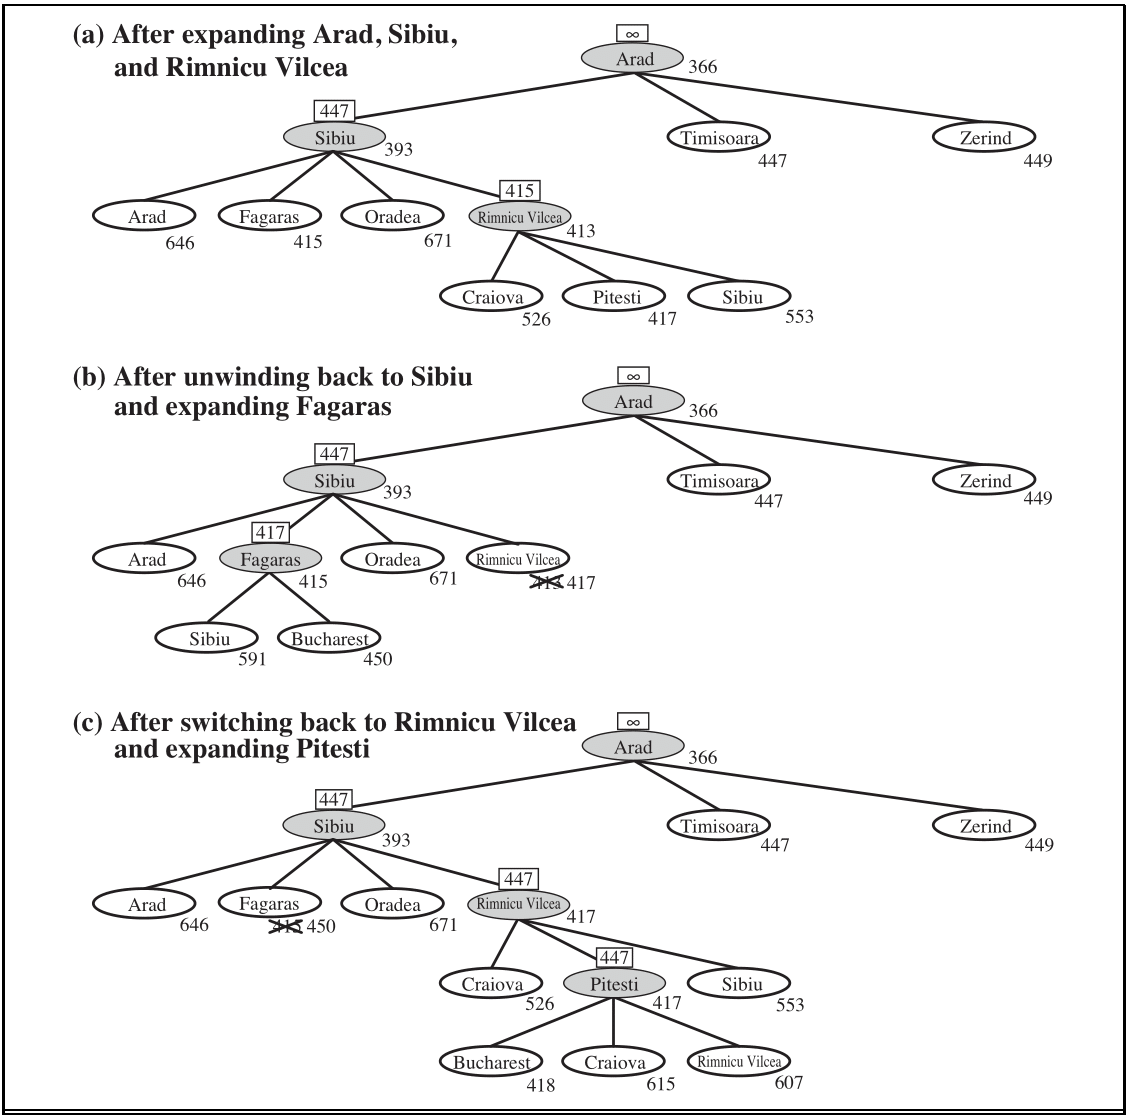
\includegraphics[width=\linewidth]{fig/rbfs.png}
    \caption{Finding a path from Arad to Bucharest by using recursive best-first search. The number above a node is its f-limit, and the number on the right of it is its f-value. The searching branch was switched two times. \cite{aima2020}} 
    \label{fig:rbfs}
\end{figure}

